\documentclass[tikz,border=6pt]{standalone}

\usepackage{amsmath}
\usepackage{sansmath}
\usepackage{xcolor}
\usetikzlibrary{arrows.meta,shapes.geometric}

\definecolor{coltreat}{HTML}{0066CC}
\definecolor{colout}{HTML}{D62828}
\definecolor{collatent}{HTML}{A6A6A6}
\definecolor{filllatent}{HTML}{F2F2F2}

\begin{document}
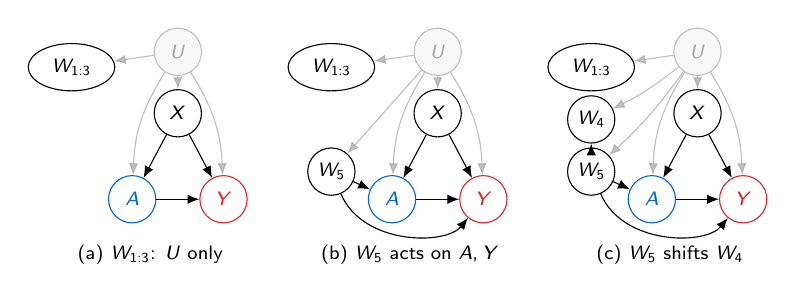
\begin{tikzpicture}[
  x=1cm,
  y=0.78cm,
  >={Latex[width=1.2mm,length=1.5mm]},
  font=\sffamily\sansmath\scriptsize,
  varnode/.style={draw,circle,inner sep=0mm,minimum size=6mm,
    font=\sffamily\sansmath\scriptsize},
  observed/.style={varnode,draw=black,text=black,fill=white},
  latent/.style={varnode,draw=collatent,draw opacity=0.72,text=collatent,
    fill=filllatent,fill opacity=0.55,text opacity=1},
  treatment/.style={varnode,draw=coltreat,text=coltreat,fill=white},
  outcome/.style={varnode,draw=colout,text=colout,fill=white},
  bnode/.style={observed,shape=ellipse,minimum width=11mm,minimum height=6mm},
  observed edge/.style={->,draw=black,line width=0.4pt},
  latent edge/.style={->,draw=collatent,opacity=0.72,line width=0.4pt},
  panellabel/.style={align=center,font=\sffamily\sansmath\scriptsize}
]

% Panel (a): the clean blocks alone.
\begin{scope}[xshift=0cm]
  \node[latent]    (Ua)  at ( 0.00, 1.85) {$U$};
  \node[observed]  (Xa)  at ( 0.00, 0.85) {$X$};
  \node[bnode]     (W3a) at (-1.35, 1.60) {$W_{1:3}$};
  \node[treatment] (Aa)  at (-0.58,-0.55) {$A$};
  \node[outcome]   (Ya)  at ( 0.58,-0.55) {$Y$};

  \draw[latent edge] (Ua) -- (W3a);
  \draw[latent edge] (Ua) -- (Xa);
  \draw[latent edge] (Ua) to[bend right=15] (Aa);
  \draw[latent edge] (Ua) to[bend left=15]  (Ya);
  \draw[observed edge] (Xa) -- (Aa);
  \draw[observed edge] (Xa) -- (Ya);
  \draw[observed edge] (Aa) -- (Ya);

  \node[panellabel] at (-0.35,-1.45) {(a) $W_{1:3}$: $U$ only};
\end{scope}

% Panel (b): add the block that acts on treatment and outcome.
\begin{scope}[xshift=3.30cm]
  \node[latent]    (Ub)  at ( 0.00, 1.85) {$U$};
  \node[observed]  (Xb)  at ( 0.00, 0.85) {$X$};
  \node[bnode]     (W3b) at (-1.35, 1.60) {$W_{1:3}$};
  \node[observed]  (W5b) at (-1.35,-0.10) {$W_5$};
  \node[treatment] (Ab)  at (-0.58,-0.55) {$A$};
  \node[outcome]   (Yb)  at ( 0.58,-0.55) {$Y$};

  \draw[latent edge] (Ub) -- (W3b);
  \draw[latent edge] (Ub) -- (Xb);
  \draw[latent edge] (Ub) -- (W5b);
  \draw[latent edge] (Ub) to[bend right=15] (Ab);
  \draw[latent edge] (Ub) to[bend left=15]  (Yb);
  \draw[observed edge] (Xb) -- (Ab);
  \draw[observed edge] (Xb) -- (Yb);
  \draw[observed edge] (Ab) -- (Yb);
  \draw[observed edge] (W5b) -- (Ab);
  \draw[observed edge] (W5b) .. controls (-0.95,-1.30) and (0.10,-1.30) .. (Yb);

  \node[panellabel] at (-0.35,-1.45) {(b) $W_5$ acts on $A,Y$};
\end{scope}

% Panel (c): add the block that W5 shifts.
\begin{scope}[xshift=6.60cm]
  \node[latent]    (Uc)  at ( 0.00, 1.85) {$U$};
  \node[observed]  (Xc)  at ( 0.00, 0.85) {$X$};
  \node[bnode]     (W3c) at (-1.35, 1.60) {$W_{1:3}$};
  \node[observed]  (W4c) at (-1.35, 0.75) {$W_4$};
  \node[observed]  (W5c) at (-1.35,-0.10) {$W_5$};
  \node[treatment] (Ac)  at (-0.58,-0.55) {$A$};
  \node[outcome]   (Yc)  at ( 0.58,-0.55) {$Y$};

  \draw[latent edge] (Uc) -- (W3c);
  \draw[latent edge] (Uc) -- (Xc);
  \draw[latent edge] (Uc) to[bend left=6] (W4c);
  \draw[latent edge] (Uc) to[bend left=6] (W5c);
  \draw[latent edge] (Uc) to[bend right=15] (Ac);
  \draw[latent edge] (Uc) to[bend left=15]  (Yc);
  \draw[observed edge] (Xc) -- (Ac);
  \draw[observed edge] (Xc) -- (Yc);
  \draw[observed edge] (Ac) -- (Yc);
  \draw[observed edge] (W5c) -- (W4c);
  \draw[observed edge] (W5c) -- (Ac);
  \draw[observed edge] (W5c) .. controls (-0.95,-1.30) and (0.10,-1.30) .. (Yc);

  \node[panellabel] at (-0.35,-1.45) {(c) $W_5$ shifts $W_4$};
\end{scope}

\end{tikzpicture}
\end{document}
